\documentclass[12pt,t]{beamer}
\usepackage{graphicx}
\setbeameroption{hide notes}
\setbeamertemplate{note page}[plain]
\usepackage{listings}

% header.tex: boring LaTeX/Beamer details + macros

% get rid of junk
\usetheme{default}
\beamertemplatenavigationsymbolsempty
\hypersetup{pdfpagemode=UseNone} % don't show bookmarks on initial view


% font
\usepackage{fontspec}
\setsansfont
  [ ExternalLocation = fonts/ ,
    UprightFont = *-regular ,
    BoldFont = *-bold ,
    ItalicFont = *-italic ,
    BoldItalicFont = *-bolditalic ]{texgyreheros}
\setbeamerfont{note page}{family*=pplx,size=\footnotesize} % Palatino for notes
% "TeX Gyre Heros can be used as a replacement for Helvetica"
% I've placed them in fonts/; alternatively you can install them
% permanently on your system as follows:
%     Download http://www.gust.org.pl/projects/e-foundry/tex-gyre/heros/qhv2.004otf.zip
%     In Unix, unzip it into ~/.fonts
%     In Mac, unzip it, double-click the .otf files, and install using "FontBook"

% named colors
\definecolor{offwhite}{RGB}{255,250,240}
\definecolor{gray}{RGB}{155,155,155}

\ifx\notescolors\undefined % slides
  \definecolor{foreground}{RGB}{255,255,255}
  \definecolor{background}{RGB}{24,24,24}
  \definecolor{title}{RGB}{107,174,214}
  \definecolor{subtitle}{RGB}{102,255,204}
  \definecolor{hilit}{RGB}{102,255,204}
  \definecolor{vhilit}{RGB}{255,111,207}
  \definecolor{lolit}{RGB}{155,155,155}
\else % notes
  \definecolor{background}{RGB}{255,255,255}
  \definecolor{foreground}{RGB}{24,24,24}
  \definecolor{title}{RGB}{27,94,134}
  \definecolor{subtitle}{RGB}{22,175,124}
  \definecolor{hilit}{RGB}{122,0,128}
  \definecolor{vhilit}{RGB}{255,0,128}
  \definecolor{lolit}{RGB}{95,95,95}
\fi
\definecolor{nhilit}{RGB}{128,0,128}  % hilit color in notes
\definecolor{nvhilit}{RGB}{255,0,128} % vhilit for notes

\newcommand{\hilit}{\color{hilit}}
\newcommand{\vhilit}{\color{vhilit}}
\newcommand{\nhilit}{\color{nhilit}}
\newcommand{\nvhilit}{\color{nvhilit}}
\newcommand{\lolit}{\color{lolit}}

% use those colors
\setbeamercolor{titlelike}{fg=title}
\setbeamercolor{subtitle}{fg=subtitle}
\setbeamercolor{institute}{fg=lolit}
\setbeamercolor{normal text}{fg=foreground,bg=background}
\setbeamercolor{item}{fg=foreground} % color of bullets
\setbeamercolor{subitem}{fg=lolit}
\setbeamercolor{itemize/enumerate subbody}{fg=lolit}
\setbeamertemplate{itemize subitem}{{\textendash}}
\setbeamerfont{itemize/enumerate subbody}{size=\footnotesize}
\setbeamerfont{itemize/enumerate subitem}{size=\footnotesize}

% page number
\setbeamertemplate{footline}{%
    \raisebox{5pt}{\makebox[\paperwidth]{\hfill\makebox[20pt]{\lolit
          \scriptsize\insertframenumber}}}\hspace*{5pt}}

% add a bit of space at the top of the notes page
\addtobeamertemplate{note page}{\setlength{\parskip}{12pt}}

% default link color
\hypersetup{colorlinks, urlcolor={hilit}}

\ifx\notescolors\undefined % slides
  % set up listing environment
  \lstset{language=bash,
          basicstyle=\ttfamily\scriptsize,
          frame=single,
          commentstyle=,
          backgroundcolor=\color{darkgray},
          showspaces=false,
          showstringspaces=false
          }
\else % notes
  \lstset{language=bash,
          basicstyle=\ttfamily\scriptsize,
          frame=single,
          commentstyle=,
          backgroundcolor=\color{offwhite},
          showspaces=false,
          showstringspaces=false
          }
\fi

% a few macros
\newcommand{\bi}{\begin{itemize}}
\newcommand{\bbi}{\vspace{24pt} \begin{itemize} \itemsep8pt}
\newcommand{\ei}{\end{itemize}}
\newcommand{\ig}{\includegraphics}
\newcommand{\subt}[1]{{\footnotesize \color{subtitle} {#1}}}
\newcommand{\ttsm}{\tt \small}
\newcommand{\ttfn}{\tt \footnotesize}
\newcommand{\figh}[2]{\centerline{\includegraphics[height=#2\textheight]{#1}}}
\newcommand{\figw}[2]{\centerline{\includegraphics[width=#2\textwidth]{#1}}}


%%%%%%%%%%%%%%%%%%%%%%%%%%%%%%%%%%%%%%%%%%%%%%%%%%%%%%%%%%%%%%%%%%%%%%
% end of header
%%%%%%%%%%%%%%%%%%%%%%%%%%%%%%%%%%%%%%%%%%%%%%%%%%%%%%%%%%%%%%%%%%%%%%

% title info
\title{R/qtl: Just barely sustainable}
\author{\href{http://kbroman.org}{Karl Broman}}
\institute{Biostatistics \& Medical Informatics, UW{\textendash}Madison}
\date{\href{http://kbroman.org}{\tt \scriptsize \color{foreground} kbroman.org}
\\[-4pt]
\href{https://github.com/kbroman}{\tt \scriptsize \color{foreground} github.com/kbroman}
\\[-4pt]
\href{https://twitter.com/kwbroman}{\tt \scriptsize \color{foreground} @kwbroman}
\\[2pt]
\scriptsize {\lolit Slides:} \href{http://bit.ly/UseR2016}{\tt \scriptsize
  \color{foreground} bit.ly/UseR2016}
}


\begin{document}

% title slide
{
\setbeamertemplate{footline}{} % no page number here
\frame{
  \titlepage

  \vfill \hfill 
\includegraphics[height=6mm]{Figs/cc-zero.png} \vspace*{-1cm}

  \note{These are slides for a talk that I will give at the UseR 2016
    conference at Stanford on 28 June 2016.

    Source: {\tt https://github.com/kbroman/Talk\_UseR2016} \\
    Slides: {\tt http://bit.ly/UseR2016\_nonotes} \\
    With notes: {\tt http://bit.ly/UseR2016}

    Also see the related paper, Broman KW (2014) Fourteen years of
    R/qtl: Just barely sustainable. J Open Res Softw 2(1):e11
    {\tt http://doi.org/10.5334/jors.at}
}
} }


\begin{frame}[c]{}

\figw{Figs/rqtl_lines_code.pdf}{1.0}

\note{
  I've been developing and maintaining an R package, R/qtl, since
  2000. The idea was conceived the week before R version 1.0 was
  released.

  This plot shows the growth of R/qtl over time. It's currently about
  60\% R code and 40\% C code.

  The Rd files were basically constructed by hand. Oog.
}
\end{frame}


\begin{frame}[c]{}

\vspace*{-1mm} \hspace*{-2mm}
\figw{Figs/inbredmice.jpg}{1.2}

\note{
I'll start with a bit of background; hopefully I can get through this
really quickly.

I focus on genetics problems, and particularly on mouse genetics.

I think these are SWR mice; the photo is from David Threadgill.
}

\end{frame}


\begin{frame}{}

\vspace*{18mm}

\centerline{
\begin{minipage}[t]{50mm}
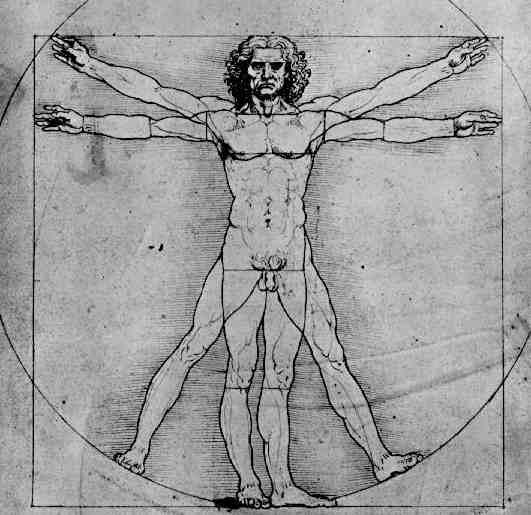
\includegraphics[height=50mm]{Figs/da-vinci-man.jpg}
\end{minipage}
\hspace{15mm}
\begin{minipage}[t]{50mm}
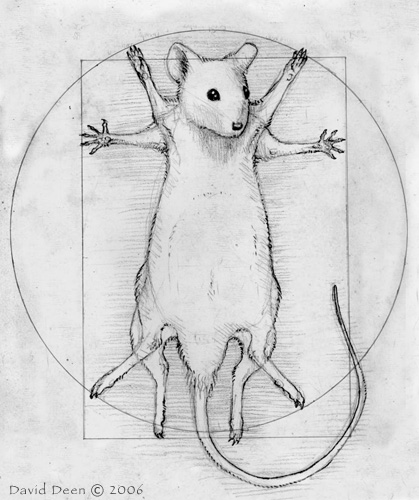
\includegraphics[height=50mm]{Figs/vitruvian_mouse.jpg}
\hspace{5mm}
\href{http://daviddeen.com}{\scriptsize \lolit \tt daviddeen.com}
\end{minipage}
}


\note{
Mice are not humans, but you can learn a great deal about human
biology and disease from mice.

The figure on the right is from David Deen.
}
\end{frame}


\begin{frame}[c]{Intercross}

\figh{Figs/intercross.pdf}{1.0}

\note{
  I've mostly focused on simple crosses between two inbred strains.

  Say strain P$_1$ has low blood pressure and P$_2$ has high blood
  pressure. We cross the two strains to get the F$_1$ hybrid, and then
  intercross F$_1$ siblings to get a large set of F$_2$
  individuals.

  The F$_2$ mice may inherit a P$_1$ or P$_2$ chromosome
  intact, but generally their chromosomes are a mosaic of the two
  parental chromosomes as a result of recombination at meiosis.  The
  points of exchange are called crossovers or recombination events.

  At any one autosomal locus, the F$_2$ individuals will have genotype
  BB, BR, or RR. We'd generate many such mice and then determine their
  genotype along chromosomes as well as measure their phenotype (e.g.,
  blood pressure). The simplest analyis is to look for genomic regions
  where genotype is associated with phenotype.
}
\end{frame}


\begin{frame}[c]{QTL mapping}

\vspace{5mm}
\only<1 | handout 0>{\figh{Figs/lodcurve_insulin.pdf}{0.9}}
\only<2>{\figh{Figs/lodcurve_insulin_with_effects.pdf}{0.9}}

\note{
  Our goal is to identify quantitative trait loci (QTL): regions of
  the genome for which genotype is associated with the phenotype.

  The basic analysis is to consider each locus, one at a time, split
  the mice into the three genotype groups, and perform analysis of
  variance.

  We then plot a test statistic that indicates the strength of the
  genotype-phenotype association.  For historical reasons, we
  calculate a LOD score as the test statistic: the log$_{10}$
  likelihood ratio comparing the hypothesis that there's a QTL at that
  position to the null hypothesis of no QTL anywhere.

  Large LOD scores indicate evidence for QTL and correspond to there
  being a difference in the phenotype average for the three genotype
  groups.
}
\end{frame}


\begin{frame}[c]{R/qtl}

\figw{Figs/rqtl_lines_code.pdf}{1.0}

\note{
  Back to this R/qtl package...

  The goal was to have a comprehensive package for this sort of
  genetic analysis in model organisms.

  We were particularly interested in having it be flexible and
  extendible: a platform for implementing new methods.
}

\end{frame}


\begin{frame}[c]{}

\centerline{\Large Good things}

\note{
  After 15 years, it becomes hard to identify things that you like
  about a software package.

  But there are good things in R/qtl: some of the code, much of the
  basic user interface design, it's comprehensive, there's lots of
  good diagnostics data visualizations, and it can be quite flexible.

  And it seems to work.
}

\end{frame}


\begin{frame}[c]{}

\centerline{\Large Bad things}

\note{
  It's easier to identify bad things.

  It's remarkable that it works, because there are basically no
  tests.  As we'll see, there's some really bad code, and lots of repeated
  code. And I've had a lot of problems with memory management,
  particularly in copying large data sets when passed from R to C. And
  the code is full of if/else statements related to cross types. And
  the data structures can be really complicated, and they've not been
  well documented at all.
}

\end{frame}

\begin{frame}[c,fragile]{Stupidest code ever}

\begin{center}
\begin{minipage}[c]{9.3cm}
\begin{semiverbatim}
\lstset{basicstyle=\normalsize}
\begin{lstlisting}[linewidth=9.3cm]
n <- ncol(data)
temp <- rep(FALSE,n)
for(i in 1:n) {
  temp[i] <- all(data[2,1:i]=="")
  if(!temp[i]) break
}
if(!any(temp)) stop("...")
n.phe <- max((1:n)[temp])
\end{lstlisting}
\end{semiverbatim}
\end{minipage}
\end{center}

\note{
  This is the stupidest code ever.

  It's basically trying to find the first non-blank element in a
  vector of character strings.

  See more discussion at
  {\tt kbroman.wordpress.com/2011/08/17/the-stupidest-r-code-ever}
}
\end{frame}


\begin{frame}[c]{Input file}

\figh{Figs/datafile.pdf}{0.6}

\note{
  This is what the basic input data file looks like. That last bit of
  code was trying to find the first non-blank element in the second
  line.

  Users had reported that with lots of phenotypes, it was taking hours
  to load their files. I thought, ``Well, you've got lots of
  phenotypes.'' But then the first time that I had lots of phenotypes,
  I realized there was a problem.

  A file might take 60 seconds to load, and 58 of those seconds were
  spent in trying to find the first non-blank character in the second
  line. Urp.
}

\end{frame}


\begin{frame}[c]{}

  \large

  {\hilit Open source} {\lolit means}

  everyone can see my stupid mistakes

  \bigskip \bigskip \bigskip

  \onslide<2>{
    {\hilit Version control} {\lolit means}

  everyone can see every stupid mistake I've ever made
}

  \note{
    They're both still totally worth it.
    }
\end{frame}


\begin{frame}[c]{More typically bad code}

  \large
      The {\hilit \tt scantwo()} function is {\hilit 1446 lines} long.

      \bigskip \bigskip

      The related C code is 20\% of the C code in R/qtl.


\note{
  This sort of thing really needs to be broken up into smaller pieces.

  As it is, it's really hard to extend and maintain.
}
\end{frame}



\begin{frame}[c]{Baroque data structures}

  \large
      {\tt attr(mycross\$geno[["X"]]\$probs, "map")}


\note{
  The data structures in R/qtl really got out of control: far too
  deeply nested.

  Attributes can be great, but when I learned about them, I started to
  pile all sorts of shit in there.
}
\end{frame}


\begin{frame}[c]{}

  \only<1>{
    \centerline{\Large User support}}

  \only<2|handout 0>{
    \centerline{\Large ``I tried X and it didn't work.''}}

  \only<3|handout 0>{
    \large ``Could you look at the attached 25-page Word
      document containing code and output and tell me if I'm doing
      something wrong?''}

  \note{
    It's great to have one's software used, but answering their
    questions requires considerable patience.

    Questions often have too little detail or far too much detail.

    I'd hope to build a ``community'' of people answering each other's
    questions, but it continues to be largely me doing the answering.

    Part of that, I think, is due to the way I use Google Groups: I
    filter all questions (to avoid spam), and in doing so, I tend to
    then just answer the questions right away. So by the time that others see the
    question, I've already answered it.

    I try hard to be patient with, and to not be offended by, users
    seeking help. I'll now often let things sit for a day or two
    before answering.
    }
\end{frame}


\begin{frame}[c]{}

  \centerline{\Large Incorporating others' code}

  \note{
    It's great to get contributions from others. But once you've incorporated
    their features, you're responsible for maintaining and supporting
    it.

    I now think that big things should mostly be made to be separate
    packages.
  }
\end{frame}


\begin{frame}[c]{}

  \centerline{\Large Version control}

  \note{
    How on earth did I get by before git?

    Really critical for incorporating others' changes, and for trying out
    new things without breaking what's working.
  }
\end{frame}


\begin{frame}[c]{}

  \centerline{\Large Unit tests and TravisCI}

  \note{
    How on earth does any of this work?

    I'm now thoroughly in love with unit tests and
    Hadley's testthat.
  }
\end{frame}


\begin{frame}[c]{R/qtl2: Let's not make the same mistakes}

  \bbi
\item C++ and Rcpp
\item testthat
\item A single ``switch'' for cross type
\onslide<2>{
\item Split into multiple packages
\item Yet another data input format
\item Flatter data structures, but still complex
}
\ei

  \note{
    I'm in the process of completing re-implementing R/qtl to better
    handle high-dimensional data and more complex crosses.

    Rcpp is totally awesome, as is testthat.

    And I've designed things so that there's just one ``switch'' for
    cross type (an object factory in C++).

    But I had the idea to split the package into multiple packages,
    and I'm not totally sure that was a good idea.

    And I have yet another data input format, and I'm still fighting
    to keep my data structures from being outlandish.

    It seems to me that there's a trade-off in complexity of the user
    interface and of the data structures.
  }
\end{frame}



\begin{frame}[c]{Summary}

  \begin{itemize}
  \itemsep12pt
  \item Sustainable software
    \bi
    \item Easier if you are your primary user
    \ei
  \item Take care of your users
    \bi
    \item Answer each question as if it's the first
    \item Primary goal is to be helpful
    \item Write many focused vignettes solving real problems
    \ei
  \item Version control
  \item Tests
  \end{itemize}

  \note{
    It's always good to include a summary.
}
\end{frame}



\begin{frame}[c]{Acknowledgments}

  \bbi
\item R/qtl users
  \item Gary Churchill, \'Saunak Sen, Hao Wu, Pjotr Prins, Danny
    Arends, Brian Yandell, Robert Corty, Timoth\'ee Flutre, Ritsert Jansen
  Lars Ronnegard, Rohan Shah, Laura Shannon, Quoc Tran, Aaron
  Wolen
\item NIH/NIGMS
\ei

  \note{
    A lot of people have contributed to R/qtl, and certainly users
    have been very kind to me.
}


\end{frame}




\begin{frame}[c]{}

\Large

Slides: \href{http://bit.ly/UseR2016}{\tt bit.ly/UseR2016} \quad

\includegraphics[height=5mm]{Figs/cc-zero.png}

\vspace{10mm}

\href{http://kbroman.org}{\tt kbroman.org}

\vspace{10mm}

\href{https://github.com/kbroman}{\tt github.com/kbroman}

\vspace{10mm}

\href{https://twitter.com/kwbroman}{\tt @kwbroman}


\note{
  Here's where you can find me, as well as the slides for this talk.
}
\end{frame}




\end{document}
